\chapter{Resultados}




\section{Sistema de cifrado}

\subsection{Inversión de Bits}


Una vez que el sistema de cifrado recibe un paquete RTP, se dealiza uno  de los pasos que conforman el algoritmo propuesto:  diffuse and destroy the meaning of compressed codeword sequence and meke it impractial to predict the original codeword sequence. Para lograr esto, se propone la inversión da al menos un bit cada  $BF = F \cdot Av \cdot MEPS$ bits, donde $Av$ es el tamaño promedio de los códigos de Huffman, MEPL is the calculated Mean Average Propagation Length (MEPL) in codeword units, $Av \cdot MEPL$ es el promedio del error de propagación en bits, y $f$ is a tunable security factor with values $ \frac{1}{MEPL}  \leq f \leq \frac{3}{4}$. Para este rango de $f$, $Av \leq BF \leq Av \cdot MEPL$ esto es, al menos un bit es invertido per average Huffman codeword size ($Av$) up to $\frac{3}{4}(Av \cdot MEPL)$ bits. Esto es lo que hace nuestro system scalable secured, as $f$ gets smaller more bits are flipoed per  $BF$-bits units increasing de system security. Depending of the specific needs of the user, $f$ provides a tradeoff between security and performance.

The actual locariton $B_{i}$ del bit a ser invertido en el flujo es calculado como sigue:

\begin{equation}
B_{i}= \left( rand   \lceil \log_{2}(f \cdot Av \cdot MEPL)  \rceil \mod{BF}      \right) +1
\end{equation}

donde $rand(Numero_bits)$ is our own designed PRNG function describes in the previous section. EL argumento $ \lceil \log_{2}(f \cdot Av \cdot MEPL)  \rceil$ representa la longitud de bits of the requested random number with límites $1 \leq B_{i} \leq BF$.

The algoritm for random bit flipping in the payload P of size $P_{s}$ bytes es outlined in the following:

PONGO ALGORITMO CON LA LIBRERIA ALGORITM2e

Ahora, para lograr una mayor robustez en este paso, es importante tomar en cuenta las siguientes consideraciones:

\begin{enumerate}
\item Primer esquema. Nueva posición con referencia al inicio del bloque (gap can be considerable).

La figura ~\ref{rtp} muestra este esquema.

\begin{figure}[H]
\centering
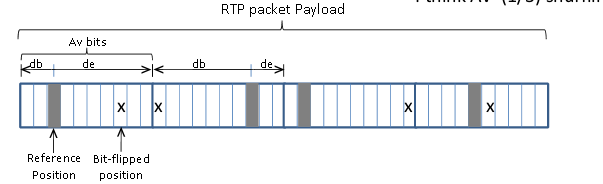
\includegraphics[width=7cm]{logos/es1.png}
\caption{Esquema 1.}
\label{eee1}
\end{figure}



\item Segundo esquema. En esta alternativa, la nueva posici[on es elegida con respecto a el $x$ previo. Esto asegura que cada uno de los bits invertidos no tienen una separación mayor de $Av$ bits. El total de bits invertidos puede ser más alto que el promedio $Av$.


La figura ~\ref{rtp} muestra el segundo esquema.

\begin{figure}[H]
\centering
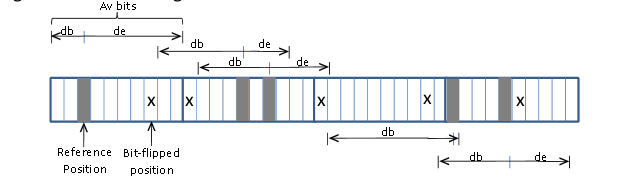
\includegraphics[width=7cm]{logos/es2.png}
\caption{Esquema 2.}
\label{eee2}
\end{figure}

A continuación se hacen algunas especificaciones para la comprensión del proceso de inversión de bits.

\begin{enumerate}
\item \textbf{db} Es el número de bits que están antes del bit de referencia.
\item \textbf{de} Es el número de bits que están después del bit de referencia.
\item \textbf{Av} El el tamaño promedio de los códigos de HUffman. Este valor se calcula por medio de la siguiente expresión:


\begin{equation}
Av = \sum_{i=1}^{N} P(C_{I})* L(C_{i}) 
\end{equation}


\end{enumerate}



\end{enumerate}



\subsection{Segment shuffling}

Después de que ha crecido el  proceso de inversión de bits, ahora, es necesario permutar los RTP-packet payload by performing an L-way shuffling. Here the payload is divided into L segmentes which are schuffled using the algorithm described below and ilustrate in figure ~\ref{shuffling}

\begin{figure}[H]
\centering
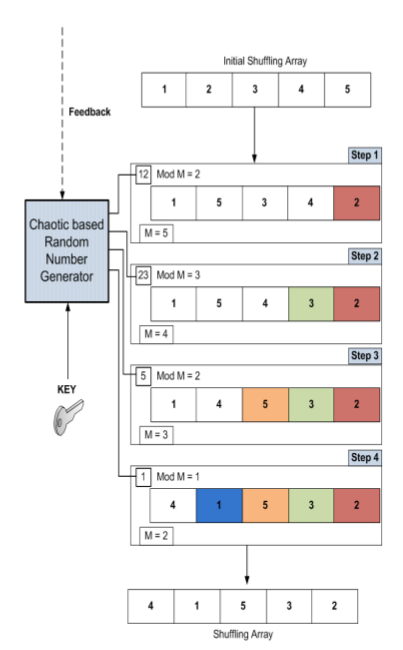
\includegraphics[width=7cm]{logos/per.png}
\caption{Esquema de permutacion.}
\label{shuffling}
\end{figure}


\subsection{Esquema robusto contra un ataque diferencial}

EL problema con el esquema de inversión de bits es que el punto de referencia del cual el número aleatorio es utilizado para invertir el bit es conocido (de el primer bit invertido la referencia es el inicio del paquete y se incrementa en Av bits), así, la idea es la siguiente: (cambiar el bit cada  $f*Av$ bits, $0 < f \leq 1$):

\begin{enumerate}
\item Elegimos una posición aleatoria ($Pos = randomChaoticNumber \mod{Av}$) de los primeros $Av$ bits in el paquete y calcular la distancia de este punto al inicio y final del bloque (en bits), ''db'' y ''de'' respectivamente.

\item Si el número aleatorio es par: $flipbitPos = (randomNumber \mod{db})$; por lo tanto $flipbitPos = Av - (randomNumber \mod{de})$. Esto es, de la posición aleatoria lanzamos una moneda (par o impar) para decidir acerca de la dirección de la inversión de bits.


\item El siguiente punto puede tomar dos direcciones, o puede ocurrir una combinación de ambos.

\begin{enumerate}
\item Ir hacia el siguiente block y repetir los pasos 1 y 2 (el inicio del siguiente blok es el nuevo punto globar de la referencia para el siguiente cálculo para la inversión del nuevo bit). EL inconveniente de este método es el espacio dejado entre bits invertidos, este puede ser más bien que $Av$ (pero como un promedio la tasa de bits invertidos es $Av$).




\item La posición del último bit invertido es el nuevo punto de referencia para el siguiente bit invertido, y se repiten los pasos 1 y 2. Para considerar la difusión del punto de referencia en la iteración actual se realiza el siguiente cálculo:

\begin{equation}
Pos = (Prev_randomChaoticNumber+new_randomChaoticNUmber) \mod{Av}
\end{equation}

el siguiente proceso es el mismo. En este esquema, los bits invertidos se encuentran aparte por no más que $Av$ bits, esto puede necesitar iteraciones adicionals al final 
\end{enumerate}
\end{enumerate}


